%%%%%%%%%%%%%%%%%%%%%%%%%%%%%%%%%%%%%%%%%%%%%%%%%%%%%%%%
%%% Cell Reports — LaTeX manuscript
%%% Based on Cell Press template v1.10
%%% Binary-first framing (v2), STAR Methods format
%%%%%%%%%%%%%%%%%%%%%%%%%%%%%%%%%%%%%%%%%%%%%%%%%%%%%%%%

%%% =====================================================
%%% HIGHLIGHTS (upload separately; <=85 characters each)
%%% =====================================================
%%% - Temporal pseudo-RGB encoding detects viral infection from label-free microscopy
%%% - Three time-offset brightfield frames stacked as RGB resolve late-stage ambiguity
%%% - Unified temporal multi-task modeling reaches 93.5% binary detection accuracy
%%% - Temporal encoding gains up to +22 pp over single-frame at 46.5 hours
%%% - The same model also predicts infection severity and time post-infection
%%%
%%% =====================================================
%%% eTOC BLURB / IN BRIEF (upload separately; ~50 words)
%%% =====================================================
%%% Zhu et al. present a temporal pseudo-RGB encoding strategy that stacks
%%% time-offset brightfield frames as color channels, enabling standard CNNs
%%% to detect viral infection from label-free microscopy. Combined with
%%% multi-task learning, the approach maintains robust detection throughout
%%% 48 hours of VEEV infection, overcoming late-stage morphological ambiguity
%%% that causes single-frame methods to fail.
%%%
%%% =====================================================
%%% GRAPHICAL ABSTRACT (upload separately as image file)
%%% — You will need to create this in PowerPoint/Illustrator
%%% =====================================================

\documentclass[12pt,letterpaper]{article}
\usepackage[a4paper, total={7in, 10in}]{geometry}
\renewcommand{\familydefault}{\sfdefault}
\usepackage{graphicx}
\usepackage{helvet}
\usepackage{authblk}
\usepackage{hyperref}
\usepackage{amsmath}
\usepackage{amssymb}
\usepackage{booktabs}
\usepackage{multirow}
\usepackage{xcolor}
\usepackage[super,comma,sort&compress]{natbib}
\bibliographystyle{numbered}
\usepackage[right]{lineno}\linenumbers

\graphicspath{{figures/}{supplementary/}}

\makeatletter
\renewcommand{\maketitle}{\bgroup\setlength{\parindent}{0pt}
\begin{flushleft}
  \textbf{\@title}

  \@author
\end{flushleft}\egroup}
\makeatother

\title{Temporal Pseudo-RGB Encoding with Multi-Task Learning for Robust Label-Free Infection Detection in Human Brain Endothelial Cells}
\date{}

\author[1,*]{Zhengjie Zhu}
\author[2]{Stephanie Trefry}
\author[1]{Hao Lu}
\author[1]{Abbas Alili}
\author[1]{Yongxin Guo}
\author[2]{Aarthi Narayanan}
\author[1]{Metin Nafi Gurcan}

\affil[1]{Center for Artificial Intelligence Research, Wake Forest University School of Medicine, Winston-Salem, NC 27157, USA}
\affil[2]{Department of Biology, George Mason University, Fairfax, VA 22030, USA}
\affil[*]{Correspondence: Zhengjie.Zhu@wfusm.edu}

\begin{document}

\maketitle

%%%%%%%%%%%%%%%%%%%%%%%%%%%%%%%%%%%%%%%%%%
\section*{SUMMARY}
%%%%%%%%%%%%%%%%%%%%%%%%%%%%%%%%%%%%%%%%%%

Automated detection of viral infection from label-free microscopy is a critical capability for high-throughput antiviral drug screening, vaccine and neutralizing-antibody evaluation, biodefense surveillance, and basic viral-kinetics research. Existing single-frame deep-learning methods, however, lack a temporal dimension and cannot represent the dynamic nature of an unfolding infection, leading to brittle detection---most acutely during late-stage infection (40--48 hours), when extensively damaged monolayers visually resemble dense uninfected cultures.
Here, we present temporal pseudo-RGB encoding: three time-offset brightfield frames ($t{-}6$h, $t{-}3$h, $t$) are stacked as red, green, and blue channels so that morphological change appears as color variation, enabling any standard ImageNet-pretrained CNN to learn the trajectory of infection without architectural modification.
We instantiate this approach as a unified temporal multi-task model and validate it on human brain microvascular endothelial cells (HBMVEC) infected with Venezuelan equine encephalitis virus (VEEV) TC-83, a clinically relevant blood--brain-barrier model for a Category B select agent.
Using a stringent cross-well row-split protocol across three biological replicates, the unified temporal model achieves 93.5\% binary detection accuracy and a time-post-infection regression MAE of 1.34 hours (R$^2 = 0.981$), and maintains a $+$19--22 percentage-point binary advantage over the single-frame counterpart during 40--48 hours.
Stratified analysis shows that the model establishes reliable detection (AUROC $\geq$ 0.99) by 10\,h for MOI 5 and MOI 1 and by 20\,h for MOI 0.1, with per-well binary accuracy of 0.92--0.99 across infected conditions.
The same forward pass yields binary infected-versus-mock detection as the primary readout together with continuous time-since-infection estimation, supporting reliable label-free infection monitoring throughout the full experiment duration.

%%%%%%%%%%%%%%%%%%%%%%%%%%%%%%%%%%%%%%%%%%
\section*{KEYWORDS}
%%%%%%%%%%%%%%%%%%%%%%%%%%%%%%%%%%%%%%%%%%

deep learning, temporal encoding, label-free microscopy, viral infection, cytopathic effect, VEEV, blood--brain barrier, multi-task learning, infection detection, HBMVEC

%%%%%%%%%%%%%%%%%%%%%%%%%%%%%%%%%%%%%%%%%%
\section*{INTRODUCTION}
%%%%%%%%%%%%%%%%%%%%%%%%%%%%%%%%%%%%%%%%%%

Automated detection of viral infection from label-free microscopy is a critical enabling capability across modern virology: it underpins high-throughput antiviral drug screening, vaccine and neutralizing-antibody evaluation, biodefense and emerging-pathogen surveillance, and basic studies of viral kinetics.\cite{ref-morens2004emerging,ref-woolhouse2005emerging,ref-zandi2019cpe}
Brightfield microscopy is particularly attractive for these applications because it is non-invasive, compatible with continuous longitudinal imaging at high temporal resolution, and avoids the artifacts and endpoint constraints of fluorescent labels or destructive viability assays.\cite{ref-riss2016assay,ref-petkidis2023review}
Building on this, recent deep-learning approaches have demonstrated promising results for automated detection of cytopathic effects (CPE)---the cell rounding, shrinkage, and detachment that mark productive viral infection---directly from brightfield images.\cite{ref-andriasyan2021iscience,ref-petkidis2024natcomm,ref-chen2022biomedicines,ref-airvic2025}
However, all of these systems treat each frame independently and discard the temporal trajectory information that is inherent in time-lapse imaging.

The central limitation is that single-frame classifiers lack a temporal dimension and therefore cannot represent the dynamic process by which an infection develops.
This structural deficiency is most visibly exposed at late time points (40--48 hours post-infection): extensively damaged infected monolayers can paradoxically resemble dense confluent uninfected cultures when judged from a single static frame, confounding both manual scoring and automated analysis.\cite{ref-wang2020cpe,ref-hsiung1994cpe,ref-leland2007cpe}
But the underlying issue is not specific to late stages---it is that any classifier built on isolated snapshots is forced to infer a dynamic process from a static image, making detection brittle whenever the static appearance is ambiguous.
We hypothesize that encoding the \emph{trajectory} of morphological change---not just the current snapshot---can resolve this ambiguity throughout the full infection timeline.

To address this, we propose temporal pseudo-RGB encoding: three time-offset brightfield frames ($t{-}6$h, $t{-}3$h, $t$) are stacked as the red, green, and blue channels of a single pseudo-color image, so that regions undergoing morphological change appear as color shifts while static regions appear gray.
This representation allows any standard ImageNet-pretrained CNN to repurpose its learned color-processing features for temporal discrimination, without any architectural modification, additional parameters, or purpose-built temporal modules such as 3D convolutions, recurrent networks, or optical-flow estimators.
Combined with a unified multi-task training objective that jointly optimizes binary infected-versus-mock detection and continuous time-post-infection regression, the same forward pass yields a robust binary readout together with a continuous time-since-infection estimate throughout 48 hours of imaging (Figure~1).

We instantiate the approach on human brain microvascular endothelial cells (HBMVEC), which constitute a critical component of the blood--brain barrier (BBB),\cite{ref-daneman2015bbb,ref-abbott2010bbb} infected with Venezuelan equine encephalitis virus (VEEV) TC-83.
VEEV is an alphavirus classified as a Category B select agent that can traverse the BBB through infection of brain endothelial cells,\cite{ref-weaver2004veev,ref-schafer2011vee,ref-salimi2020mbio} so HBMVEC--VEEV provides a clinically relevant model for studying neurotropic viral infection dynamics in a system where reliable label-free monitoring has direct biodefense and antiviral-screening utility.

Our approach makes four contributions.
\textbf{First}, we introduce temporal pseudo-RGB encoding, an architecture-agnostic method that encodes morphological trajectory by stacking time-offset frames as pseudo-RGB channels and is compatible with any standard pretrained CNN backbone.
\textbf{Second}, using this encoding within a unified multi-task model, we demonstrate robust binary infection detection across the full 48-hour timeline---reaching 93.5\% binary accuracy overall and maintaining 97--100\% binary accuracy during 40--48 hours, where the single-frame counterpart degrades by $-$19 to $-$22 percentage points (down to 75\% at 46.5\,h).
\textbf{Third}, we provide a stratified detectability analysis quantifying when and under what conditions the model becomes reliable: per-condition AUROC analysis shows AUROC $\geq$ 0.99 first sustained at 10\,h for MOI 5 and MOI 1 and at 20\,h for MOI 0.1, and per-well binary accuracy reaches 0.92--0.99 across infected conditions; the same model also predicts time post-infection with MAE $= 1.34$\,h ($R^2 = 0.981$), enabling continuous monitoring rather than thresholded calls.
\textbf{Fourth}, we validate generalization using a stringent cross-well row-split protocol across three independent biological replicates and held-out wells, with bootstrap 95\% CIs reported throughout.

%%%%%%%%%%%%%%%%%%%%%%%%%%%%%%%%%%%%%%%%%%
\section*{RESULTS}
%%%%%%%%%%%%%%%%%%%%%%%%%%%%%%%%%%%%%%%%%%

\subsection*{Component ablation establishes the contribution of each design element}

To quantify the contribution of temporal encoding and multi-task supervision to binary infected-versus-mock detection---the primary evaluation target throughout this paper---we performed a systematic component ablation in which the two design elements are added independently to a common ResNet50 backbone (Table~1).

The single-frame binary classifier achieved 89.2\% binary accuracy.
Adding temporal encoding alone improved binary detection to 92.1\% ($+$2.9\,pp), the larger of the two single-component contributions, while adding multi-task supervision alone (single-frame with auxiliary time regression) yielded 90.7\% ($+$1.5\,pp), confirming that the auxiliary supervisory signal contributes complementary information even without temporal encoding.
Combining both, the unified temporal multi-task model reaches \textbf{93.5\% binary accuracy} (bootstrap 95\% CI $[88.4, 97.4]$; 1,000 iterations, well-level resampling, see STAR Methods) together with a time-post-infection regression MAE of 1.34\,h ($R^2 = 0.981$), and we use this unified temporal multi-task model as the comparator throughout the rest of the paper.

A binary-only multi-task variant (temporal encoding $+$ auxiliary time regression but trained without the severity head) reaches 93.2\% binary accuracy with MAE $= 1.33$\,h, slightly below the unified model's 93.5\%; we interpret this as evidence that the severity supervisory signal helps even coarse binary discrimination by encouraging the shared backbone to learn finer-grained morphological features.\cite{ref-caruana1997mtl}
For time regression, temporal encoding improves MAE from 1.67\,h to 1.34\,h and $R^2$ from 0.971 to 0.981, confirming that temporal context benefits both binary robustness and the regression secondary output.
Detailed ablation numbers for the four-class severity output across all configurations are reported in supplementary Table~S1.

\subsection*{Time-dependent detectability of viral infection}

To characterize when reliable infection detection is established and how it is sustained over time, we analyzed binary detection accuracy in 3-hour bins across the full 48-hour imaging timeline (Figure~2).

\textbf{Onset of reliable detection.}
Per-condition binary AUROC analysis (Figure~S3) shows that the unified temporal model establishes reliable detection (AUROC $\geq 0.99$, sustained across two consecutive bins) at \textbf{10 hours post-infection for MOI 5 and MOI 1}, and at \textbf{20 hours for MOI 0.1}.
Once reliable detection is established, all three conditions maintain AUROC $\geq 0.99$ through the full 46.5-hour imaging period.
The longer onset for MOI 0.1 reflects its biology: only $\sim$10\% of cells are initially infected, so visible morphological change takes longer to accumulate at the well level.
The earlier reliable detection for MOI 5 and MOI 1 is consistent with their rapid, high-titer CPE progression.

\textbf{Late-stage robustness.}
The temporal advantage is most pronounced during late-stage infection (Figure~2).
During the early phase (0--6 hours), both temporal and single-frame models perform comparably ($\sim$70\% binary accuracy), reflecting that CPE has not yet visibly manifested and that the temporal model's earlier channels are partially clamped to the experiment boundary; this interval defines a pre-onset window prior to reliable detection.
Between 7 and 36 hours, both models achieve high binary accuracy ($>$93\%), with temporal encoding providing marginal improvement as CPE actively develops.
During the late phase (40--48 hours), the two models diverge sharply: the single-frame model degrades to 75--80\% binary accuracy, while the temporal model maintains 97--100\% binary accuracy.
At 43.5 hours, the temporal model achieves 100\% binary accuracy compared to 80.6\% for the single-frame model ($+$19.4\,pp); at 46.5 hours, the advantage reaches $+$22.5\,pp (97.5\% vs.\ 75.0\%).

This late-stage degradation of the single-frame model is attributable to high-confluency morphological ambiguity: extensively damaged infected monolayers share visual features with dense mock cultures when viewed in isolation.
The temporal model resolves this ambiguity by encoding the \emph{trajectory} of morphological change---a progressively deteriorating monolayer produces distinct color patterns in the pseudo-RGB representation compared to a stably confluent culture.
This combination of early detection (by 10--20\,h depending on MOI) and sustained late-stage robustness is essential for practical applications such as antiviral screening, where reliable readouts are required across the full duration of an experiment.

\subsection*{MOI-dependent detectability of viral infection}

To characterize how reliably the unified temporal model detects infection across viral dose levels, we report per-well binary detection accuracy stratified by MOI and biological replicate (Figure~3).
Across the 12 held-out test wells (3 biological replicates $\times$ 4 conditions, single well per condition per run after the row-split protocol), the unified temporal model achieves the following binary accuracies:

\begin{itemize}
  \item \textbf{MOI~5}: 0.92, 0.98, 0.97 across Runs 1--3 (mean 0.957);
  \item \textbf{MOI~1}: 0.99, 0.96, 1.00 (mean 0.983);
  \item \textbf{MOI~0.1}: 0.99, 0.83, 0.71 (mean 0.843);
  \item \textbf{Mock}: 0.98, 0.92, 0.96 (mean 0.953).
\end{itemize}

Binary detection accuracy is high across most wells ($\geq$0.91 for 10 of 12 wells), with the lowest values concentrated in the MOI~0.1 column (range 0.71--0.99), consistent with the subtler and more heterogeneous CPE phenotype expected at low viral dose.
Mock wells achieve consistently high accuracy (0.92--0.98) across all three biological replicates, demonstrating that the model does not generate excess false positives.
Combined with the time-to-detection analysis above (10\,h for MOI 5/1, 20\,h for MOI 0.1), this stratified view delineates the practical operating envelope of the model: it is reliable across the full duration of the experiment for moderate-to-high MOI conditions, and remains useful---though more variable across biological replicates---at the low-MOI condition where CPE is sparse and delayed.

As a secondary supervisory signal, the unified temporal model also produces a four-class severity readout (MOI~5 vs.\ MOI~1 vs.\ MOI~0.1 vs.\ mock) which serves principally to enrich the shared backbone with finer-grained morphological features; the overall and per-time-window four-class confusion matrices are reported in supplementary Figures~S5 and~S2 and supplementary Table~S1.

\subsection*{Time regression achieves high accuracy with practical utility}

As a secondary output of the unified temporal multi-task model, the regression head predicts time post-infection with MAE $= 1.34$\,h and $R^2 = 0.981$ (Figure~4).
The temporal model consistently outperforms the single-frame multi-task counterpart (MAE $= 1.67$\,h, $R^2 = 0.971$) across the timeline, with the largest advantage during early hours: at 1.5 hours post-infection, the temporal model achieves MAE $= 0.36$\,h compared to 0.83\,h for single-frame (2$\times$ improvement).
This suggests that the temporal channels provide strong time-ordering cues even when classification confidence is low, as the frame-to-frame differences encode the rate of morphological change independent of absolute appearance.
The continuous time-since-infection estimate enables monitoring use cases beyond binary thresholding---for instance, ranking wells by progression stage or aligning temporally heterogeneous experiments---using the same forward pass that produces the binary readout.

\subsection*{Feature space analysis reveals improved class separation with temporal encoding}

To visualize the effect of temporal encoding on learned representations, we computed t-SNE embeddings of backbone features from both models (Figure~S6).
The temporal model produces tighter, more clearly separated clusters for each infection condition, with distinct boundaries between infected classes and mock controls; the single-frame model shows substantial overlap between infection levels, particularly between MOI~5 and MOI~1 at late time points.
When features are colored by hours post-infection, the temporal model exhibits a smooth time gradient within each cluster, indicating that the learned representation encodes both infection status and temporal progression---consistent with the multi-task training objective, which requires the shared backbone to support both classification and time regression.

\subsection*{Temporal offset ablation identifies optimal encoding span}

To investigate the effect of temporal span on detection performance, we trained the unified temporal multi-task model with three offset configurations (Table~2): short ($-$3, $-$1.5, 0\,h), standard ($-$6, $-$3, 0\,h), and long ($-$12, $-$6, 0\,h), in addition to the single-frame baseline ($0, 0, 0$\,h).

The single-frame baseline achieved 91.0\% binary accuracy.
The short-span temporal model improved to 93.0\%, the standard span to 93.5\% (best binary accuracy), and the long span to 92.2\% (best regression MAE of 1.24\,h).
The standard ($-$6, $-$3, 0\,h) configuration offers the best overall balance: it provides sufficient temporal context for late-stage discrimination while minimizing early-frame clamping artifacts.
The long-span model's superior regression performance is consistent with broader temporal context providing finer time-ordering cues, though the slight decrease in binary accuracy may reflect increased noise from spanning a wider morphological window.
All temporal spans (3--12\,h) outperform the single-frame baseline, confirming that the approach is robust to the specific choice of offset.

%%%%%%%%%%%%%%%%%%%%%%%%%%%%%%%%%%%%%%%%%%
\section*{DISCUSSION}
%%%%%%%%%%%%%%%%%%%%%%%%%%%%%%%%%%%%%%%%%%

\subsection*{Temporal encoding captures morphological trajectory and resolves late-stage ambiguity}

The most significant finding of this study is that encoding morphological trajectory---rather than static snapshots---substantially improves infection detection robustness, particularly during late-stage infection.
The $+$19--22 percentage-point binary advantage during 40--48 hours (up to $+$22 pp at 46.5 h) represents a practically meaningful performance gap for longitudinal infection monitoring.

The mechanism underlying this improvement is intuitive: in the pseudo-RGB representation, regions undergoing morphological change produce color shifts (e.g., a cell rounding over 6 hours appears as a red-to-blue gradient), while static regions appear gray.
A standard CNN trained on ImageNet has learned to exploit color patterns, and the temporal pseudo-RGB encoding repurposes this capability for temporal discrimination without any architectural modification.
Across the component comparison in Table~1, temporal encoding consistently improves binary detection across every model configuration tested, supporting the conclusion that learned features depend on morphological change over time rather than on static appearance alone.

In real-world infection monitoring scenarios---antiviral drug screening, biosafety assessment, longitudinal infection studies---reliable detection must be maintained throughout the full experiment duration, not just during the intermediate window where CPE is most visually obvious.
The single-frame model's sharp degradation after 40 hours arises from a specific biological confound: at advanced CPE stages, infected cells have largely detached or lysed, leaving a sparse debris field that, in brightfield microscopy, can resemble the dense confluent monolayer of healthy mock cultures.
The temporal model resolves this by capturing the trajectory leading to the current state: a well that has been progressively losing cells over hours looks fundamentally different in the pseudo-RGB representation from one that has maintained stable confluency, even if their current single frames are ambiguous.

Existing deep learning approaches to CPE detection---including Petkidis et al.\cite{ref-petkidis2024natcomm} (adenovirus and HSV, 88--100\% binary accuracy), Andriasyan et al.\cite{ref-andriasyan2021iscience} (adenovirus), and Chen et al.\cite{ref-chen2022biomedicines} (influenza, parainfluenza, enterovirus)---demonstrate strong binary performance but treat each frame independently, discarding the temporal trajectory inherent in time-lapse imaging.
AIRVIC\cite{ref-airvic2025} similarly operates on single frames.
Because these studies use different virus--cell systems, datasets, and evaluation protocols, the reported accuracies are not directly comparable to ours; we cite them to delineate the methodological landscape rather than to claim a head-to-head improvement.
None of these approaches have addressed late-stage morphological ambiguity, nor have they characterized when reliable detection is established as a function of viral dose and time post-infection.
The present work addresses these gaps through a unified temporal formulation that is architecturally simple and potentially extensible across virus systems, and through a stratified per-MOI, per-time detectability analysis that delineates the practical operating envelope of label-free infection monitoring.

The simplicity of pseudo-RGB encoding is a deliberate design choice rather than a limitation.
Brightfield microscopy images are inherently grayscale (single-channel); pseudo-RGB encoding stacks three time-offset frames into a three-channel image that directly matches the input format expected by standard ImageNet-pretrained CNNs.
This repurposes the color-processing capabilities already learned from natural images for temporal discrimination, without requiring purpose-built temporal architectures such as 3D convolutional networks, recurrent models, or optical flow estimators.
Such architectures require substantially more data and training infrastructure and offer no interpretability advantage over the pseudo-RGB approach, which makes morphological change directly visible as color variation in the input.
The temporal offset ablation (Table~2) confirms that the approach is robust to offset choice, with the 3--12 hour span all outperforming the single-frame baseline.

\subsection*{Multi-task supervision improves binary detection through complementary signal}

The component ablation reveals that temporal encoding is the dominant contributor to binary detection improvement, while multi-task supervision (auxiliary time regression and a severity head) provides a smaller but consistent additional gain.
Empirically, the unified temporal multi-task model's binary accuracy (93.5\%) slightly exceeds the binary-only temporal multi-task variant (93.2\%), consistent with the view that the auxiliary supervisory signals encourage the shared backbone to learn finer-grained morphological features that benefit even coarse binary discrimination.\cite{ref-caruana1997mtl}
The mechanism is intuitive: requiring the backbone to also predict continuous time post-infection and to distinguish dose levels forces it to represent the rate and stage of morphological change, not just the binary infected/uninfected distinction.

Our model is intentionally unified rather than a dedicated binary classifier: a single forward pass produces (1) the primary binary infected-versus-mock readout and (2) a continuous time-since-infection estimate.
This formulation supports downstream analysis needs---such as ranking wells by progression stage or temporally aligning experiments---without maintaining separate models, while preserving binary detection as the headline result.

\subsection*{Limitations of the study}

Several limitations should be acknowledged.
First, while validated across three independent biological replicates, all experiments used the same HBMVEC passage range and VEEV TC-83 vaccine strain. Generalization to virulent VEEV strains, other alphaviruses, or different cell types requires further investigation.
Second, binary detection at the lowest viral dose (MOI~0.1) is more variable across biological replicates (per-well accuracy 0.71--0.99) than at higher doses, reflecting the biological reality that only $\sim$10\% of cells are initially infected and CPE accumulation is heterogeneous and delayed; the multi-task severity supervisory signal does not yet yield practically actionable MOI-level classification (supplementary Table~S1).
Third, temporal encoding requires sequential imaging data and introduces a latency of 6 hours before full three-channel input is available; for the initial frames, clamped padding reduces effective temporal information.
Fourth, the fixed temporal offsets ($-$6, $-$3, 0\,h) may not be optimal across all virus--cell systems; adaptive offset selection could be explored in future work.
Fifth, infection labels are assigned at the well level based on experimental conditions; individual cells within infected wells may remain uninfected, particularly at low MOI, and orthogonal single-cell validation (e.g., immunofluorescence) was not performed.
Finally, all reported numbers come from a single random seed; uncertainty is quantified by well-level bootstrap rather than repeated training runs, so training-time variance is not separately characterized.

%%%%%%%%%%%%%%%%%%%%%%%%%%%%%%%%%%%%%%%%%%
\section*{RESOURCE AVAILABILITY}
%%%%%%%%%%%%%%%%%%%%%%%%%%%%%%%%%%%%%%%%%%

\subsection*{Materials availability}

This study did not generate new unique reagents.

\subsection*{Data and code availability}

\begin{itemize}
  \item Microscopy image data reported in this paper are not publicly available because of confidentiality restrictions associated with the underlying study materials.
  \item All original code has been deposited at GitHub (\url{https://github.com/CAIR-LAB-WFUSM/cell_tempo}) and is publicly available as of the date of publication.
\end{itemize}

%%%%%%%%%%%%%%%%%%%%%%%%%%%%%%%%%%%%%%%%%%
\section*{ACKNOWLEDGMENTS}
%%%%%%%%%%%%%%%%%%%%%%%%%%%%%%%%%%%%%%%%%%

The authors thank the members of the Gurcan and Narayanan laboratories for helpful discussions and technical support.
This work was supported by [funding agency, grant number(s) to be inserted before submission]. The funders had no role in study design, data collection and analysis, decision to publish, or preparation of the manuscript.

%%%%%%%%%%%%%%%%%%%%%%%%%%%%%%%%%%%%%%%%%%
\section*{AUTHOR CONTRIBUTIONS}
%%%%%%%%%%%%%%%%%%%%%%%%%%%%%%%%%%%%%%%%%%

Conceptualization, A.N., Z.Z. and M.N.G.; methodology, Z.Z.; software, Z.Z.; validation, Z.Z. and S.T.; formal analysis, Z.Z.; investigation, Z.Z. and S.T.; resources, A.N. and M.N.G.; data curation, Z.Z. and S.T.; writing---original draft preparation, Z.Z.; writing---review and editing, Z.Z., S.T., H.L., Y.G., A.N. and M.N.G.; visualization, Z.Z.; supervision, A.N. and M.N.G.; project administration, M.N.G.; funding acquisition, A.N. and M.N.G. All authors have read and agreed to the published version of the manuscript.

%%%%%%%%%%%%%%%%%%%%%%%%%%%%%%%%%%%%%%%%%%
\section*{DECLARATION OF INTERESTS}
%%%%%%%%%%%%%%%%%%%%%%%%%%%%%%%%%%%%%%%%%%

The authors declare no competing interests.

%%%%%%%%%%%%%%%%%%%%%%%%%%%%%%%%%%%%%%%%%%
\section*{DECLARATION OF GENERATIVE AI AND AI-ASSISTED TECHNOLOGIES}
%%%%%%%%%%%%%%%%%%%%%%%%%%%%%%%%%%%%%%%%%%

During the preparation of this work, the author(s) used Claude (Anthropic) in order to assist with manuscript formatting and editing. After using this tool, the author(s) reviewed and edited the content as needed and take(s) full responsibility for the content of the publication.

%%%%%%%%%%%%%%%%%%%%%%%%%%%%%%%%%%%%%%%%%%
\section*{SUPPLEMENTAL INFORMATION INDEX}
%%%%%%%%%%%%%%%%%%%%%%%%%%%%%%%%%%%%%%%%%%

\begin{description}
  \item Figure S1. Predicted infection probability over time for temporal and single-frame models, by condition
  \item Figure S2. Per-time-window four-class confusion matrices for temporal and single-frame models (0--12h, 12--24h, 24--48h)
  \item Figure S3. Per-condition binary AUROC over time for the unified temporal model, showing early detection onset and sustained reliability throughout the 48-hour imaging period
  \item Figure S4. Temporal pseudo-RGB encoding visualized as color variation: representative input channels and composite at three time points
  \item Figure S5. Four-class confusion matrices (overall and by analysis window) for the unified temporal multi-task model
  \item Figure S6. t-SNE visualization of ResNet50 backbone features for temporal vs single-frame models
  \item Figure S7. Grad-CAM attention maps for representative infected and mock test samples at two time points ($t=20$h and $t=40$h)
  \item Figure S8. Dataset hierarchy and temporal sample construction
  \item Table S1. Full component ablation including four-class severity accuracy
  \item Table S2. Full temporal offset ablation including four-class severity accuracy
\end{description}

%%%%%%%%%%%%%%%%%%%%%%%%%%%%%%%%%%%%%%%%%%
\section*{MAIN FIGURE TITLES AND LEGENDS}
%%%%%%%%%%%%%%%%%%%%%%%%%%%%%%%%%%%%%%%%%%

%%% Figure 1 — End-to-end overview schematic (was Figure S7)
\noindent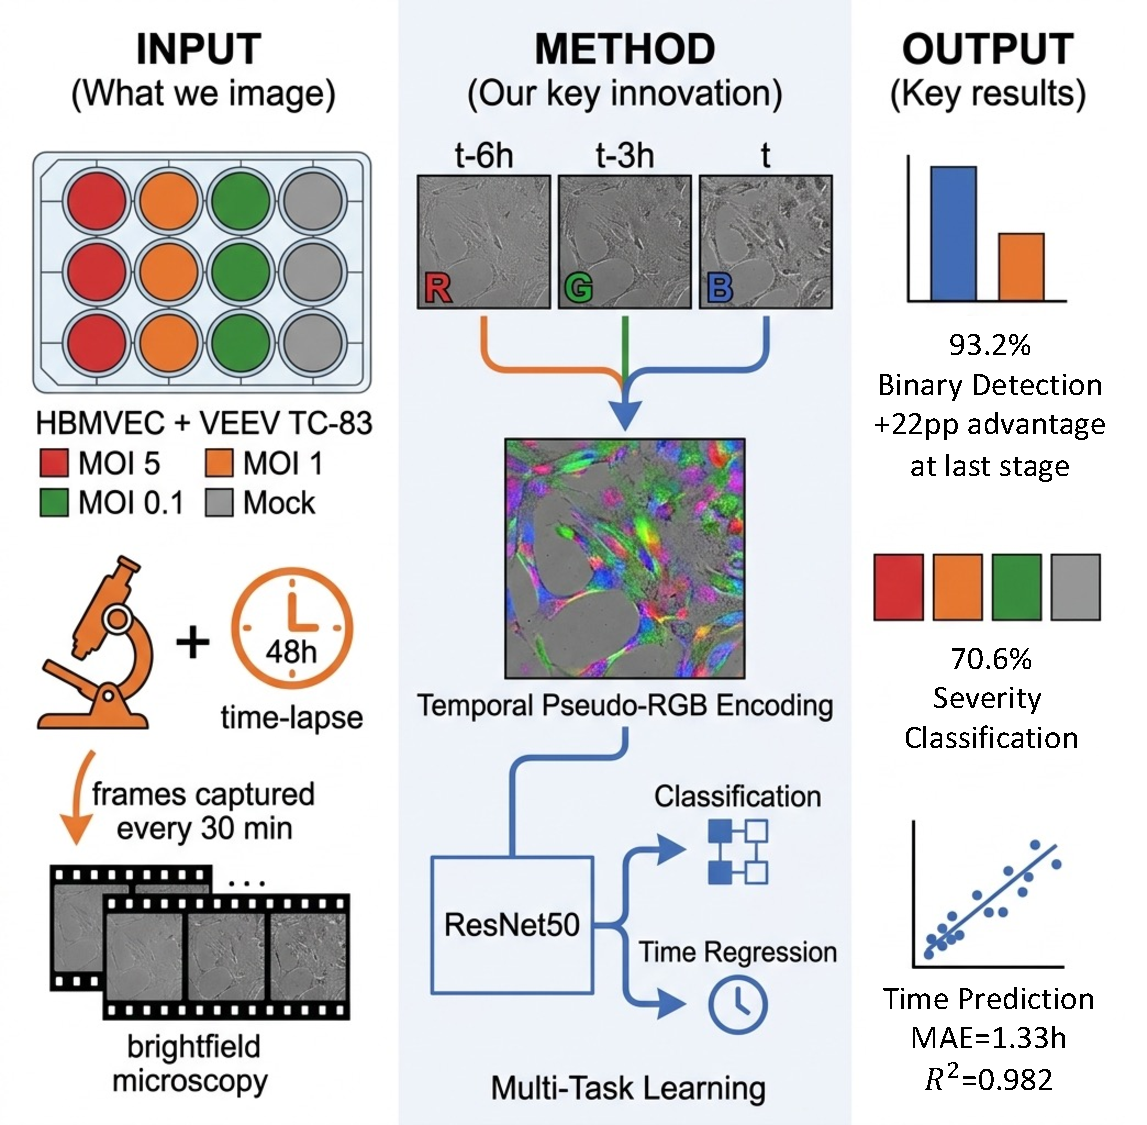
\includegraphics[width=\linewidth]{figS7_method_overview.pdf}

\subsection*{Figure 1. End-to-end overview of temporal pseudo-RGB encoding for label-free infection detection}

Study-level schematic summarizing the end-to-end workflow of this manuscript.
HBMVEC cultures infected with VEEV TC-83 at multiple MOI levels (MOI~5, MOI~1, MOI~0.1, and mock) are imaged by brightfield microscopy every 30 minutes over 48 hours.
For each time point, three time-offset frames ($t{-}6$h, $t{-}3$h, $t$) are stacked as the red, green, and blue channels of a single pseudo-color image, in which morphological change appears as color variation while static regions remain gray.
The resulting pseudo-RGB image is processed by an ImageNet-pretrained ResNet50 backbone trained as a unified multi-task network.
The primary output is robust binary infected-versus-mock detection; continuous time-post-infection regression and a four-class severity head provide secondary outputs and serve as auxiliary supervisory signals that improve binary detection.

\newpage

%%% Figure 2 — Time-dependent detectability (was Figure 3)
\noindent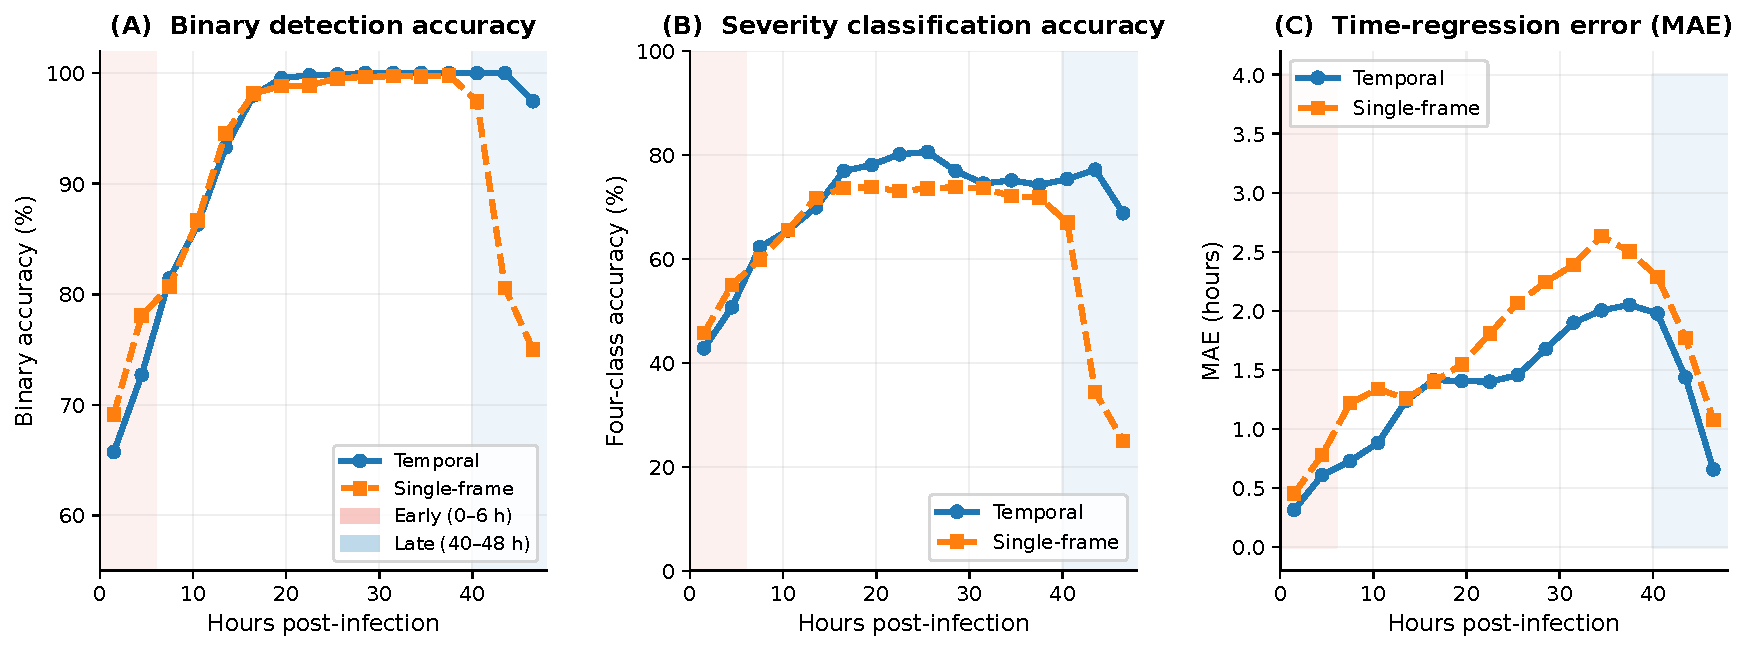
\includegraphics[width=\linewidth]{fig1_main_comparison.pdf}

\subsection*{Figure 2. Time-dependent detectability: temporal encoding maintains robust binary detection throughout 48 hours of infection}

Comparison of the unified temporal multi-task model and the single-frame multi-task counterpart across the 48-hour infection timeline.
(A) Binary (infected vs.\ mock) accuracy over time: the temporal model (blue) maintains $>$97\% binary accuracy at 40--48\,h, while the single-frame model (orange, dashed) drops to 75\%. Shaded regions mark the early phase (0--6\,h, red) and late phase (40--48\,h, blue) as defined in the text.
(B) Per-condition reliability: the four-class severity panel is provided for context; the headline result is that the temporal model sustains stable detection performance throughout the timeline, whereas the single-frame model degrades sharply at late time points.
(C) Time-regression MAE over time: the temporal model achieves consistently lower prediction error, with the largest advantage during early hours (0--6\,h) when temporal channels carry the strongest time-ordering signal.

\newpage

%%% Figure 3 — MOI-dependent detectability: per-well binary heatmap (was Figure S4)
\noindent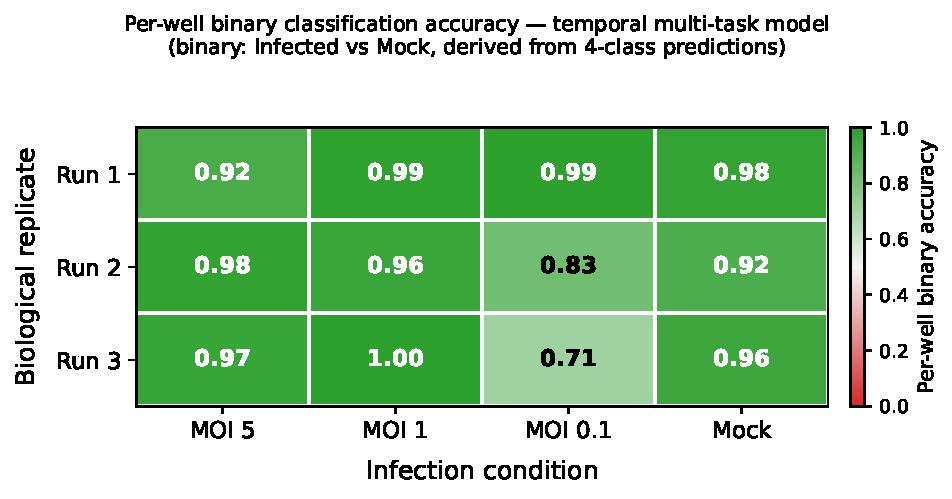
\includegraphics[width=\linewidth]{figS7_well_heatmap.pdf}

\subsection*{Figure 3. MOI-dependent detectability: per-well binary classification accuracy across biological replicates}

Heatmap of per-well binary detection accuracy (Infected vs.\ Mock) for the unified temporal multi-task model, evaluated on the 12 held-out test wells.
Wells are organized by biological replicate (rows: Run~1, Run~2, Run~3) and infection condition (columns: MOI~5, MOI~1, MOI~0.1, Mock).
Annotated values indicate per-well binary accuracy; the color scale ranges from red (low) through white to green (high).
Binary detection is high across most wells ($\geq$0.91 for 10 of 12 wells), with the lowest values concentrated in the MOI~0.1 column (range 0.71--0.99), consistent with the subtler and more heterogeneous CPE phenotype expected at low viral dose.
Mock wells achieve consistently high accuracy (0.92--0.98) across all three biological replicates, demonstrating that the model does not generate excess false positives.

\newpage

%%% Figure 4 — Time-post-infection regression scatter (was Figure 6)
\noindent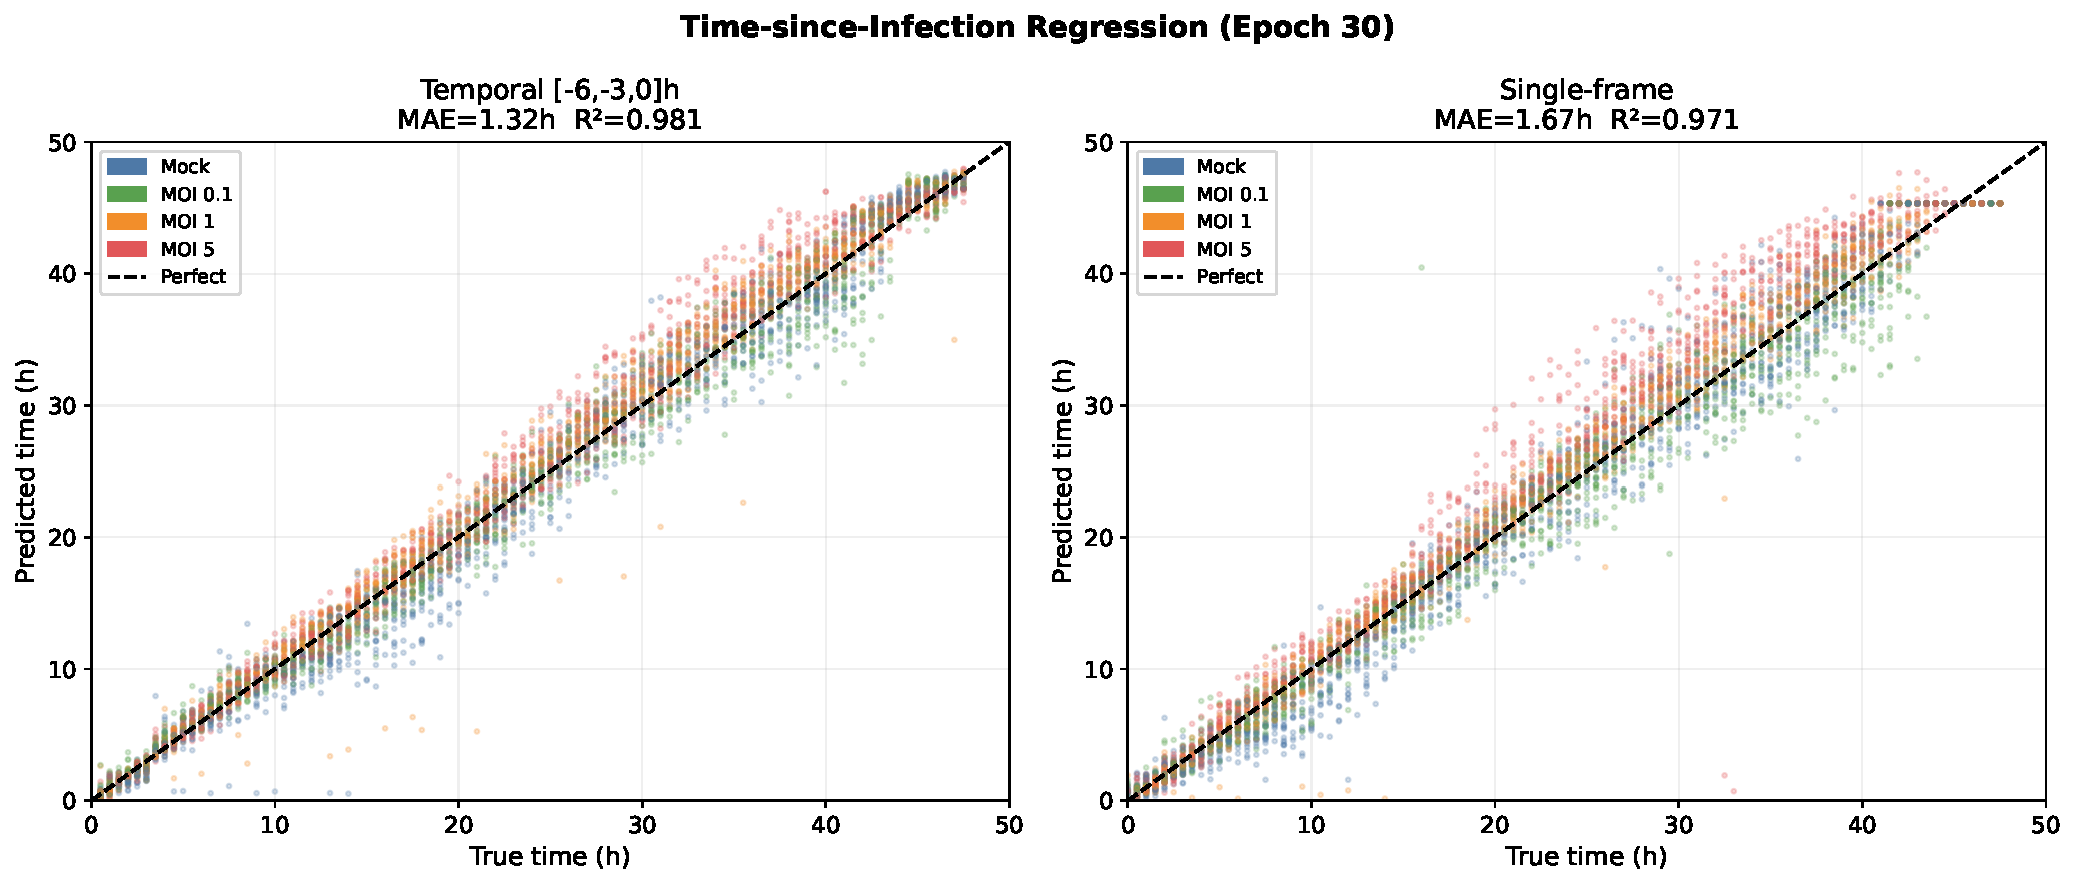
\includegraphics[width=\linewidth]{fig4_regression.pdf}

\subsection*{Figure 4. The unified temporal multi-task model accurately predicts time post-infection}

Predicted vs.\ actual time post-infection for (A) the unified temporal multi-task model (MAE $= 1.34$\,h, $R^2 = 0.981$) and (B) the single-frame multi-task counterpart (MAE $= 1.67$\,h, $R^2 = 0.971$).
Points are colored by infection condition (MOI~5, MOI~1, MOI~0.1, Mock).
The temporal model achieves tighter clustering around the diagonal, particularly during early hours (0--6\,h) where temporal channels provide strong time-ordering cues.
The dashed line indicates perfect prediction ($y = x$).

%%%%%%%%%%%%%%%%%%%%%%%%%%%%%%%%%%%%%%%%%%
\section*{SUPPLEMENTARY FIGURE LEGENDS}
%%%%%%%%%%%%%%%%%%%%%%%%%%%%%%%%%%%%%%%%%%

\newpage

%%% Figure S1 — Confidence trajectories
\noindent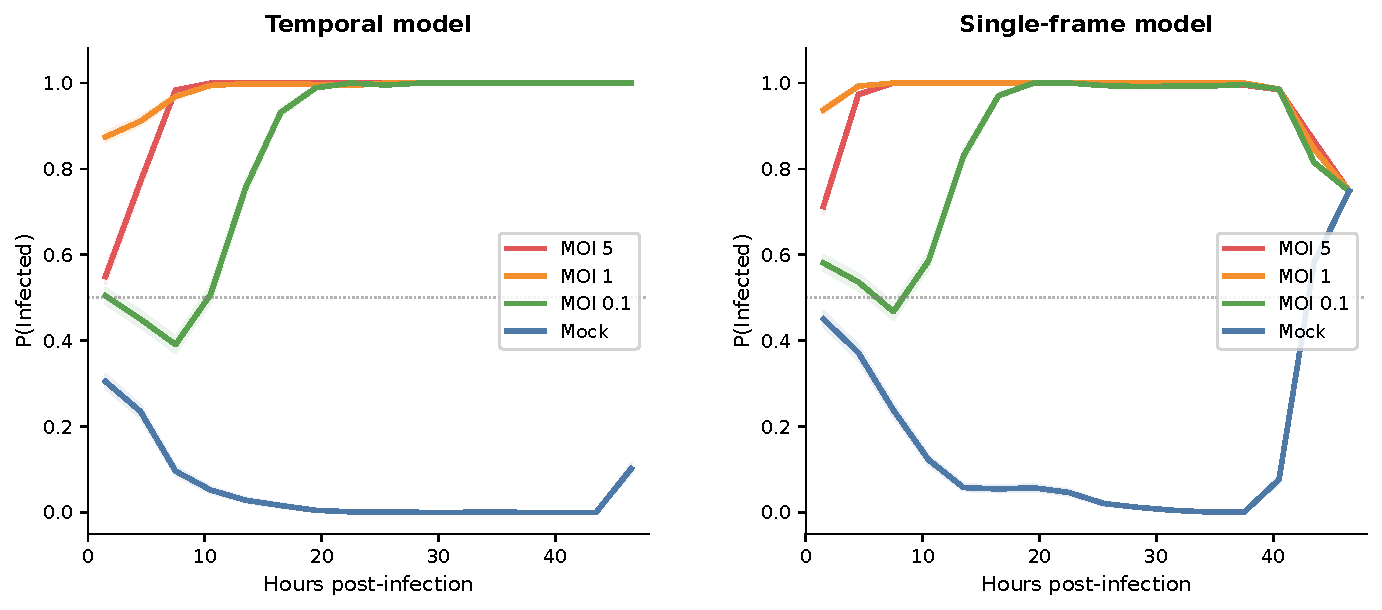
\includegraphics[width=\linewidth]{figS4_confidence_trajectories.pdf}

\subsection*{Figure S1. Predicted infection probability over time by condition}

Mean predicted P(Infected)\,=\,$1 - P(\text{Mock})$ across the 48-hour imaging period, shown separately for the temporal model (left) and single-frame model (right).
Each line represents one of the four experimental conditions (MOI~5, MOI~1, MOI~0.1, Mock); shaded bands show $\pm$1 SEM.
The dashed horizontal line marks the decision boundary ($P = 0.5$).
In the temporal model, all three infected conditions separate from Mock and stabilize above the decision boundary by approximately 10--20 hours, whereas Mock confidence remains consistently low.
In the single-frame model, this separation is less stable: infected-condition probabilities decline at late time points ($>$40h) as damaged monolayers acquire visual features similar to dense confluent Mock cultures.

\newpage

%%% Figure S2 — Per-time-window confusion matrices
\noindent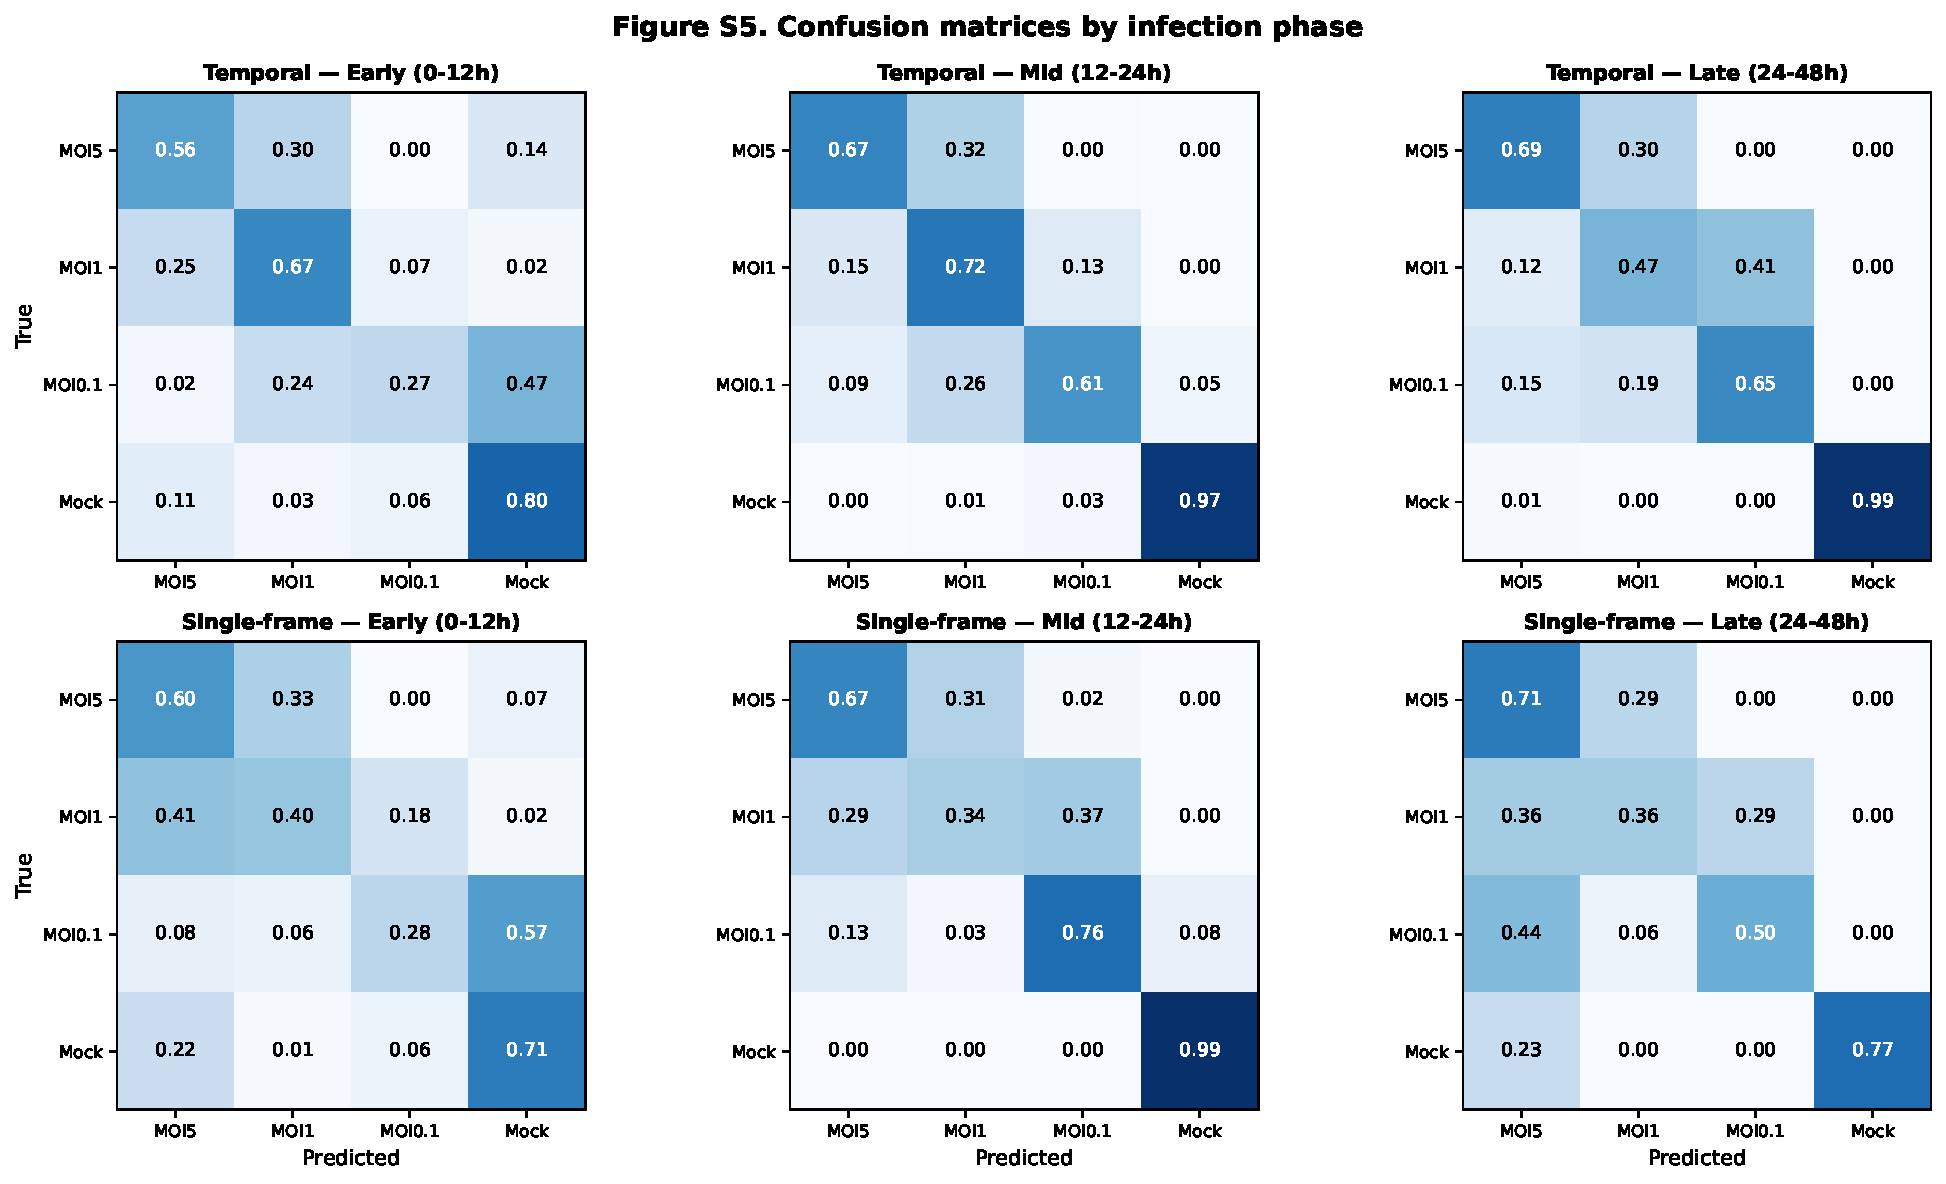
\includegraphics[width=\linewidth]{figS5_confusion_per_phase.pdf}

\subsection*{Figure S2. Four-class confusion matrices by time window}

Row-normalized confusion matrices for the temporal model (top row) and single-frame model (bottom row), computed in three non-overlapping time windows: 0--12h, 12--24h, and 24--48h.
Values indicate the fraction of true-class samples predicted as each class (row percentages).
Both models show higher MOI~0.1 confusion during 0--12h, reflecting the sparse initial infection in low-dose wells.
In the 24--48h window, the temporal model maintains robust discrimination across all four conditions, whereas the single-frame model shows increased Mock confusion for infected classes---consistent with the late-stage morphological ambiguity described in the main text.

\newpage

%%% Figure S3 — Per-condition AUROC over time (temporal model only)
\noindent
\includegraphics[width=\linewidth]{figS6_auroc_over_time.pdf}

\subsection*{Figure S3. Per-condition detection reliability throughout the 48-hour infection timeline}

Binary AUROC (infected condition vs Mock) computed in 3-hour bins across the full imaging period for the unified temporal multi-task model.
Three panels correspond to the three infected conditions (MOI~5, MOI~1, MOI~0.1), each evaluated against Mock controls.
The dashed horizontal line marks AUROC\,=\,0.99; shaded regions indicate time bins exceeding this threshold.
Vertical dotted lines indicate the earliest time bin at which AUROC\,$\geq$\,0.99 is first sustained across two consecutive bins.
MOI~5 reaches reliable detection earliest owing to rapid, high-titer CPE progression, while MOI~0.1 requires more time as only a fraction of cells are initially infected.
Once reliable detection is established, all three conditions maintain AUROC\,$\geq$\,0.99 through the full 46.5-hour imaging period.

\newpage

%%% Figure S4 — Temporal pseudo-RGB encoding visualized (was old main Fig 2)
\noindent\includegraphics[width=\linewidth]{fig_temporal_rgb_examples.png}

\subsection*{Figure S4. Temporal pseudo-RGB encoding visualized as color variation}

Representative temporal pseudo-RGB samples showing how temporal change in the brightfield signal manifests as color variation in the encoded image.
For each example, the three input grayscale frames at offsets $t{-}6$h, $t{-}3$h, and $t$ are shown alongside the resulting pseudo-RGB composite in which the three frames are mapped to the red, green, and blue channels respectively.
Cells undergoing morphological change between time points produce visible color shifts in the composite, while static structures appear as gray.
This encoding allows a standard ImageNet-pretrained CNN to leverage its learned color-processing features to detect temporal change without architectural modification.

\newpage

%%% Figure S5 — Four-class confusion matrices (was old main Fig 4)
\noindent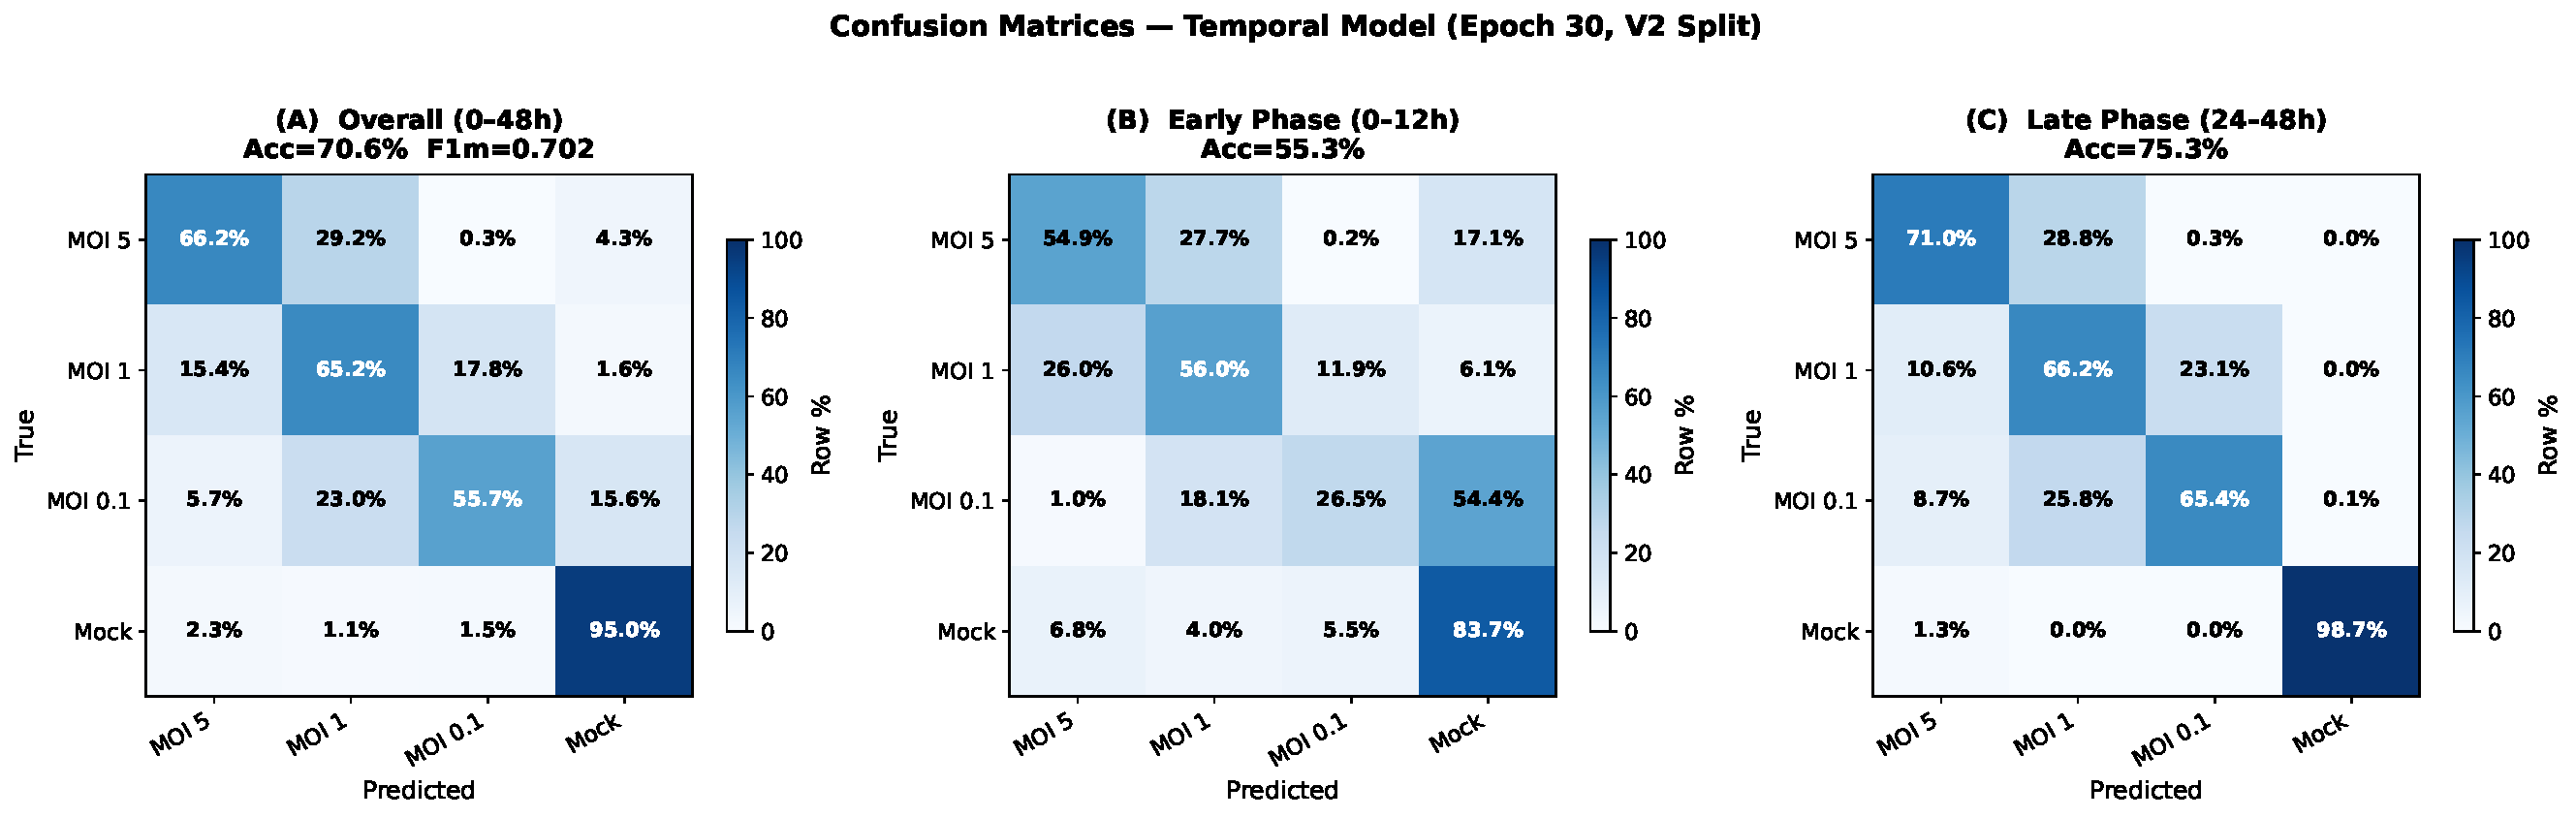
\includegraphics[width=\linewidth]{fig2_confusion_matrices.pdf}

\subsection*{Figure S5. Four-class confusion matrices for the unified temporal multi-task model}

Row-normalized confusion matrices for the four-class severity head of the unified temporal multi-task model (left) and the single-frame multi-task counterpart (right), aggregated across the full 0--48h test set.
Rows correspond to ground-truth conditions (MOI~5, MOI~1, MOI~0.1, Mock); columns correspond to predicted classes; values indicate the fraction of true-class samples assigned to each predicted class.
The temporal model improves overall four-class accuracy from 65.9\% to 70.6\%, with the largest gains on MOI~5 and Mock; MOI~1 and MOI~0.1 remain the most confused pair, consistent with the partially overlapping CPE kinetics expected for adjacent low-dose infection conditions.
The four-class severity head is reported here as a secondary output and a supervisory signal that improves the primary binary detection task; it is not the main evaluation target of the manuscript.

\newpage

%%% Figure S6 — t-SNE feature space (was old main Fig 5)
\noindent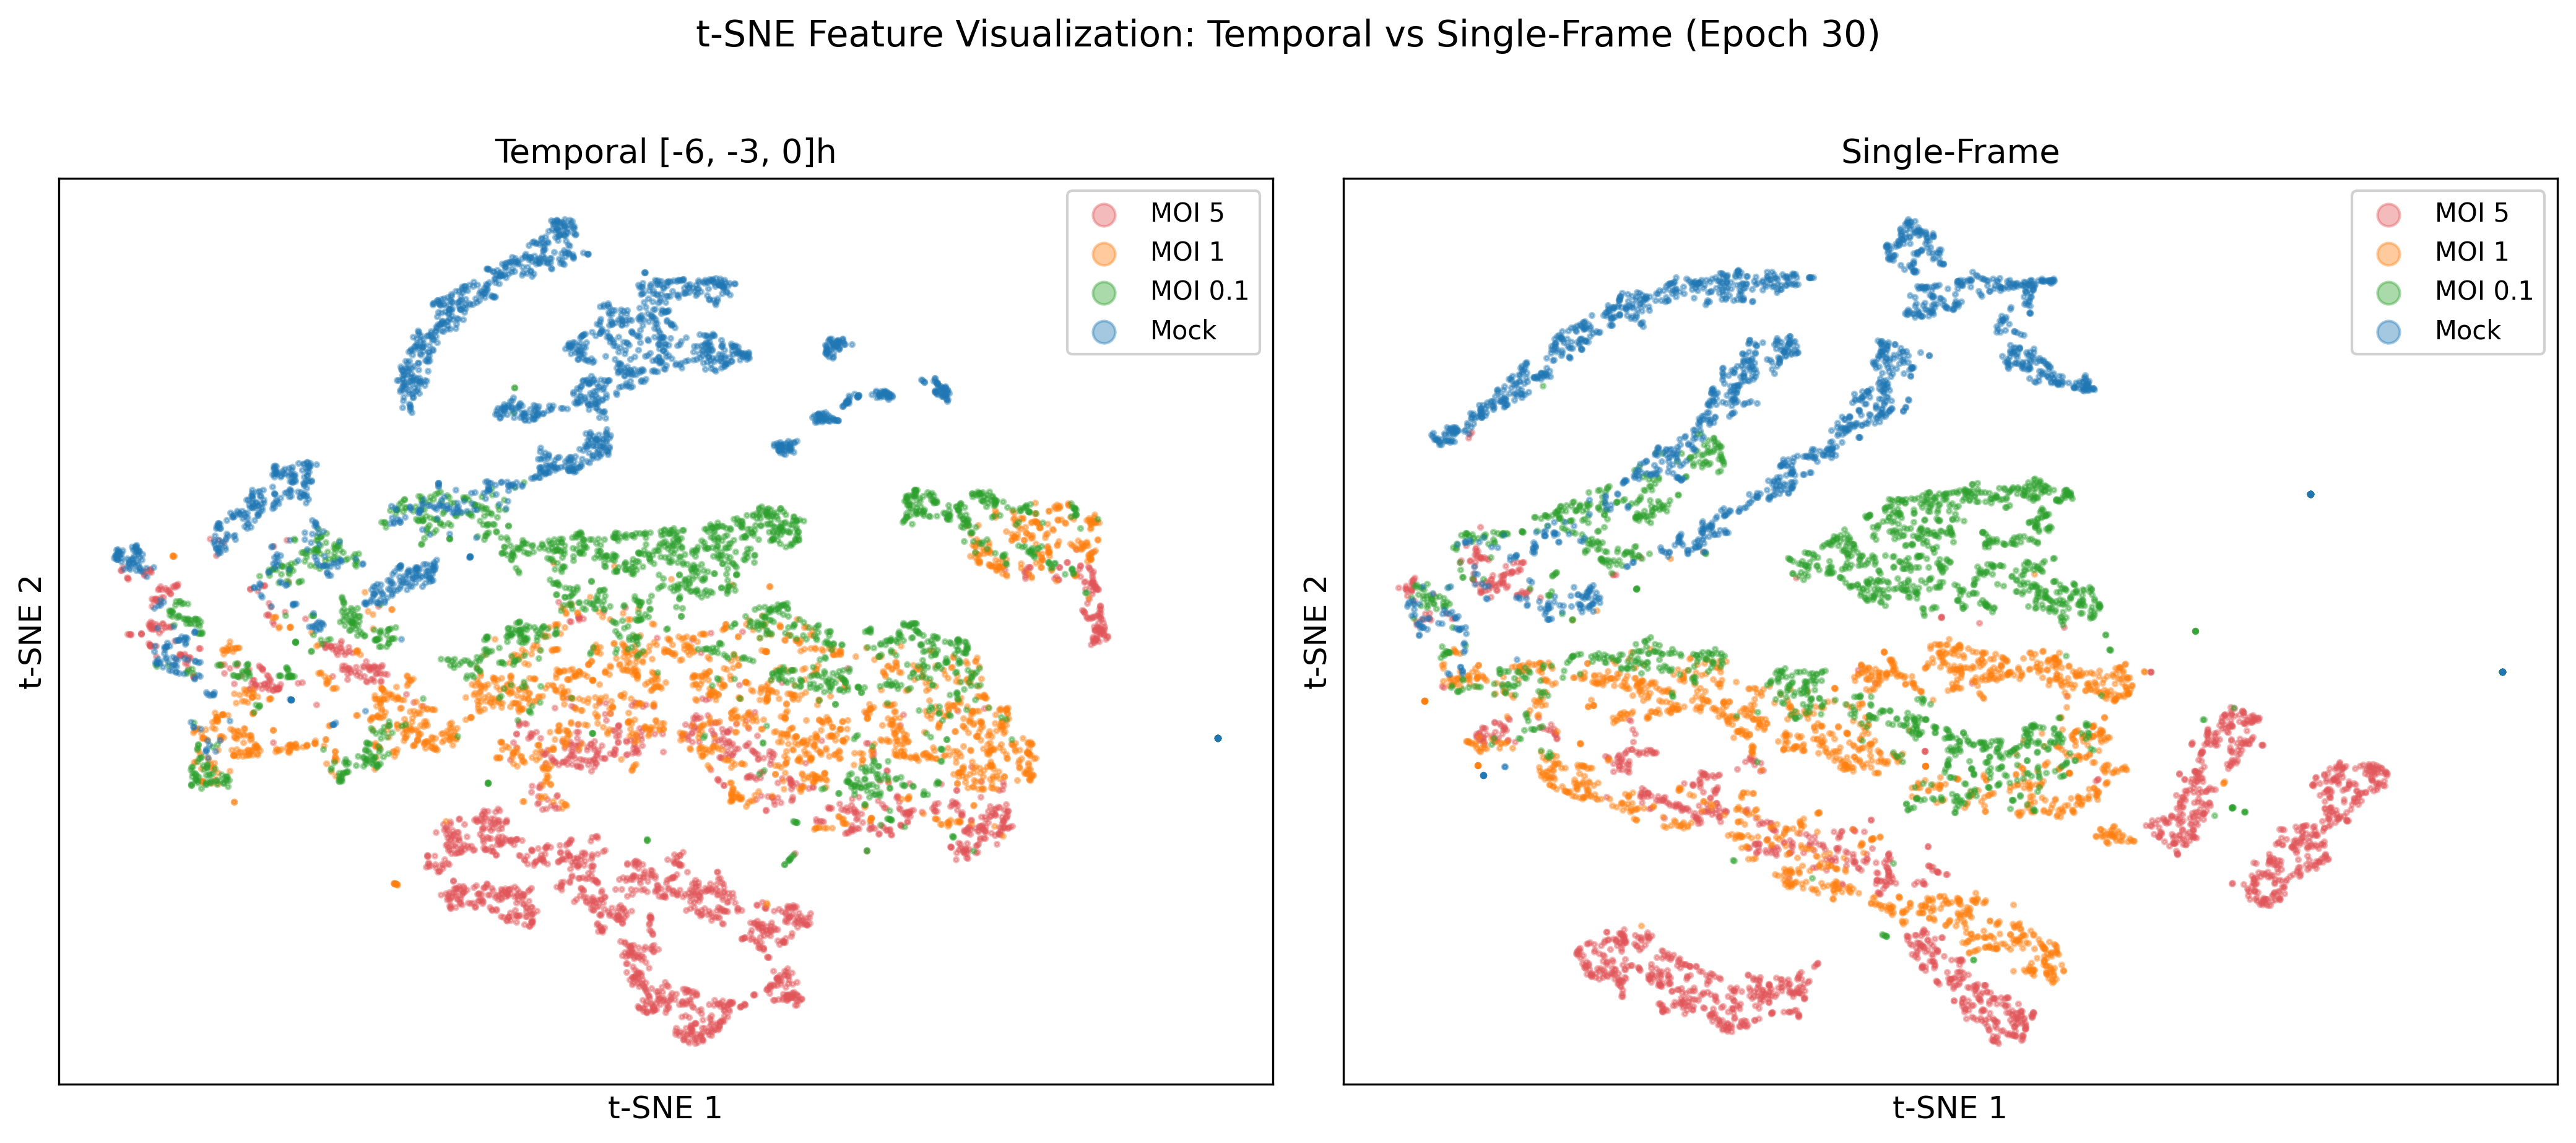
\includegraphics[width=\linewidth]{fig_tsne_temporal_vs_single.png}

\subsection*{Figure S6. t-SNE visualization of ResNet50 backbone features}

Two-dimensional t-SNE embeddings of 2{,}048-dimensional ResNet50 backbone features extracted from held-out test samples for the unified temporal multi-task model (left) and the single-frame multi-task counterpart (right).
Points are colored by ground-truth condition (MOI~5, MOI~1, MOI~0.1, Mock).
Mock samples form a tight cluster well separated from infected samples in both models; among infected conditions, the temporal model produces a more graded MOI-ordered structure, consistent with its improved binary detection and four-class severity performance.
t-SNE was computed with perplexity~30 over 1{,}000 iterations using scikit-learn defaults; this visualization is provided as qualitative context only.

\newpage

%%% Figure S7 — Grad-CAM attention maps (was old S5)
\noindent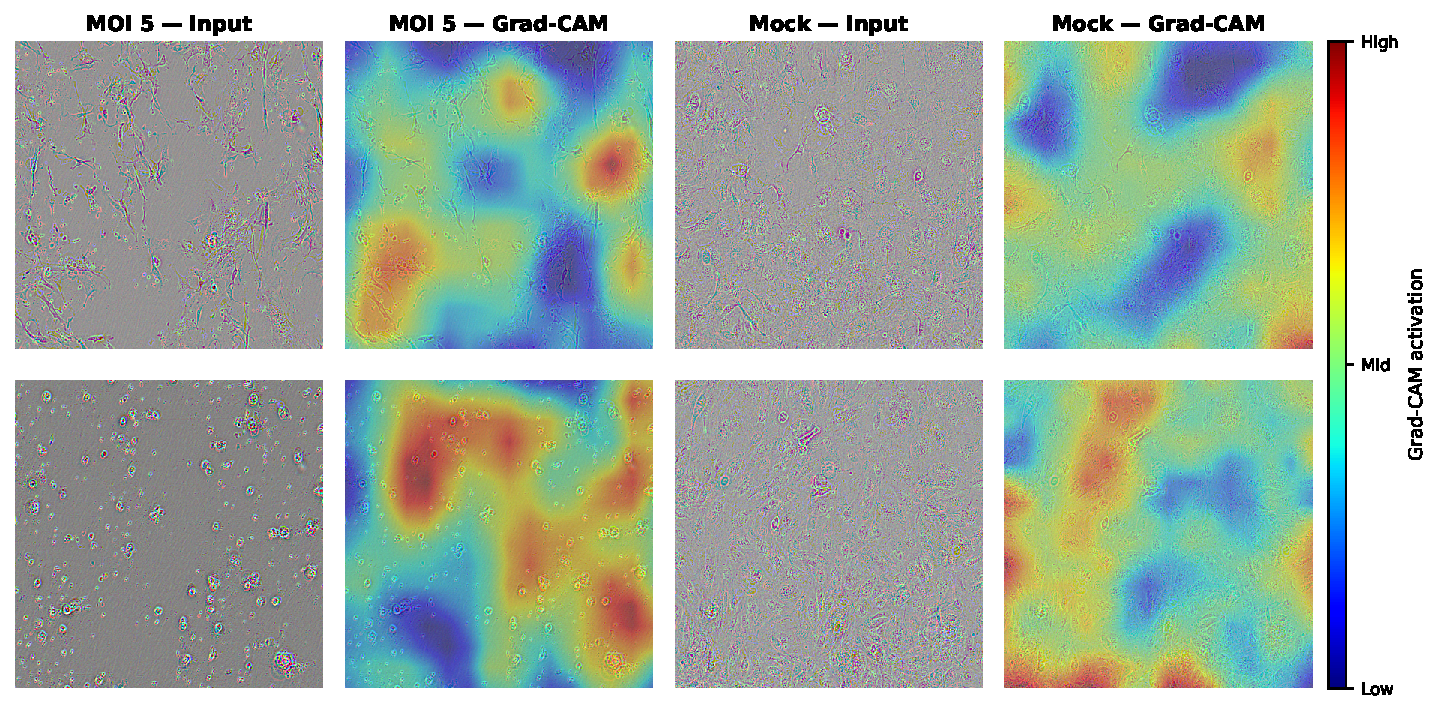
\includegraphics[width=\linewidth]{figS8_cam_attention.pdf}

\subsection*{Figure S7. Grad-CAM attention maps for representative test samples}

Gradient-weighted class activation mapping (Grad-CAM) for four representative test samples from Run~3, arranged in a $2\times4$ grid.
Rows correspond to time points (top: $t=20$h; bottom: $t=40$h); within each row, columns show: MOI~5 pseudo-RGB input, MOI~5 Grad-CAM overlay, Mock pseudo-RGB input, Mock Grad-CAM overlay.
Input images are enhanced temporal pseudo-RGB composites (R\,=\,$t{-}6$h, G\,=\,$t{-}3$h, B\,=\,$t$; per-channel percentile stretch with $\gamma=0.7$ for display clarity).
Grad-CAM activations were computed with respect to the true class using the final convolutional layer (ResNet50 \texttt{layer4}); colorbar indicates relative activation magnitude (Low--Mid--High).
All four samples were correctly classified.
The activation maps indicate that the model responds to cell-containing regions throughout the field of view, with no systematic focus on image artifacts or corners.
These patterns are provided as qualitative context for model interpretability and do not constitute evidence for specific biological mechanisms.

\newpage

%%% Figure S8 — Dataset hierarchy schematic (was old S6)
\noindent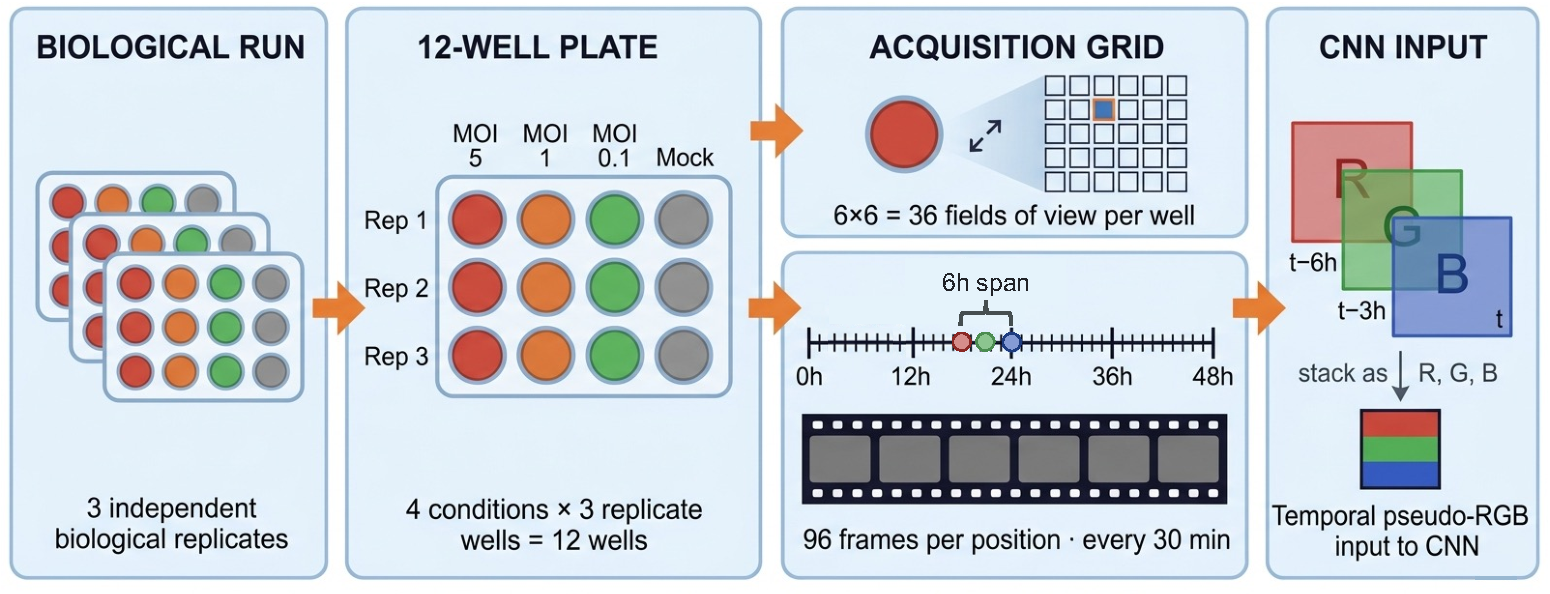
\includegraphics[width=\linewidth]{figS6_dataset_hierarchy.pdf}

\subsection*{Figure S8. Dataset hierarchy and temporal sample construction}

Schematic overview of the acquisition hierarchy used in this study.
Each biological run corresponds to one 12-well plate containing four conditions (MOI~5, MOI~1, MOI~0.1, and Mock) with three technical replicate wells per condition.
Each well is sampled on a 6$\times$6 grid of acquisition positions, and each position contributes a 96-frame brightfield time series collected every 30 minutes over 48 hours.
Temporal pseudo-RGB samples are constructed by selecting three frames at offsets $t{-}6$h, $t{-}3$h, and $t$ from each position-specific time series and stacking them as the red, green, and blue channels for the CNN input.

\newpage

%%%%%%%%%%%%%%%%%%%%%%%%%%%%%%%%%%%%%%%%%%
\section*{SUPPLEMENTARY TABLES}
%%%%%%%%%%%%%%%%%%%%%%%%%%%%%%%%%%%%%%%%%%

%%% Table S1 — Full component ablation including 4cls accuracy
\subsection*{Table S1. Full component ablation including four-class severity accuracy}

{\small\begin{tabular}{llcccccc}
\toprule
\textbf{Method} & \textbf{Task} & \textbf{Temporal} & \textbf{Multi-task} & \textbf{Bin Acc} & \textbf{4cls Acc} & \textbf{MAE (h)} & \textbf{R$^2$} \\
\midrule
\multicolumn{8}{l}{\emph{Single-frame models}} \\
SF binary cls-only & Binary & & & 89.2\% & --- & --- & --- \\
SF reg-only & Reg & & & --- & --- & 1.45 & 0.979 \\
SF binary multi-task & Binary & & \checkmark & 90.7\% & --- & 1.49 & 0.977 \\
SF four-class cls-only & 4-class & & & --- & 64.3\% & --- & --- \\
SF four-class multi-task & 4-class & & \checkmark & 91.0\%\textsuperscript{a} & 65.9\% & 1.67 & 0.971 \\

\midrule
\multicolumn{8}{l}{\emph{Temporal models}} \\
Temporal binary cls-only & Binary & \checkmark & & 92.1\% & --- & --- & --- \\
Temporal reg-only & Reg & \checkmark & & --- & --- & 1.41 & 0.979 \\
Temporal binary multi-task & Binary & \checkmark & \checkmark & \underline{93.2\%} & --- & \textbf{1.33} & \textbf{0.982} \\
Temporal four-class cls-only & 4-class & \checkmark & & --- & 68.7\% & --- & --- \\
\textbf{Unified temporal multi-task} & 4-class & \checkmark & \checkmark & \textbf{93.5\%}\textsuperscript{a} & \textbf{70.6\%} & \underline{1.34} & \underline{0.981} \\
\bottomrule
\end{tabular}}

\bigskip

Full component ablation including the four-class severity accuracy column omitted from main Table~1.
The temporal four-class result (70.6\%) is reported here as supervisory-signal evidence: it improves over the single-frame counterpart (65.9\%) by 4.7~percentage points, indicating that temporal encoding provides additional discriminative information for finer-grained MOI distinctions, but the absolute level is not yet practically actionable for MOI-level classification (see Discussion).
Bold values indicate best performance per column; underlined values indicate second-best.

\textsuperscript{a}Binary accuracy derived from four-class predictions by collapsing MOI classes 0--2 into ``Infected.''

\newpage

%%% Table S2 — Full temporal offset ablation including 4cls accuracy
\subsection*{Table S2. Full temporal offset ablation including four-class severity accuracy}

\begin{tabular}{lcccccc}
\toprule
\textbf{Offset config} & \textbf{Span} & \textbf{Bin Acc ($\uparrow$)} & \textbf{4cls Acc ($\uparrow$)} & \textbf{F1\textsubscript{macro} ($\uparrow$)} & \textbf{MAE (h) ($\downarrow$)} & \textbf{R$^2$ ($\uparrow$)} \\
\midrule
Single-frame [0, 0, 0] & 0h & 91.0\% & 65.9\% & 0.633 & 1.67 & 0.971 \\
Short [$-$3, $-$1.5, 0] & 3h & 93.0\% & 68.4\% & 0.648 & 1.45 & 0.979 \\
Standard [$-$6, $-$3, 0] & 6h & \textbf{93.5\%} & \textbf{70.6\%} & \textbf{0.703} & 1.34 & 0.981 \\
Long [$-$12, $-$6, 0] & 12h & 92.2\% & 69.1\% & 0.668 & \textbf{1.24} & \textbf{0.984} \\
\bottomrule
\end{tabular}

\bigskip

Full temporal offset ablation including the four-class severity accuracy column omitted from main Table~2.
Four-class accuracy follows the same trend as binary accuracy across offset configurations, peaking at the standard ($-$6, $-$3, 0\,h) span; absolute four-class numbers are reported here for completeness and supervisory-signal context only.

%%%%%%%%%%%%%%%%%%%%%%%%%%%%%%%%%%%%%%%%%%
\section*{MAIN TABLES, INCLUDING TITLES AND LEGENDS}
%%%%%%%%%%%%%%%%%%%%%%%%%%%%%%%%%%%%%%%%%%

\newpage

%%% Table 1 — Component ablation (binary-focused; full table with 4cls in supplementary Table S1)
\subsection*{Table 1. Component ablation: contribution of temporal encoding and multi-task supervision to binary detection}

{\small\begin{tabular}{llccccc}
\toprule
\textbf{Method} & \textbf{Task} & \textbf{Temporal} & \textbf{Multi-task} & \textbf{Bin Acc} & \textbf{MAE (h)} & \textbf{R$^2$} \\
\midrule
\multicolumn{7}{l}{\emph{Single-frame models}} \\
SF binary cls-only & Binary & & & 89.2\% & --- & --- \\
SF reg-only & Reg & & & --- & 1.45 & 0.979 \\
SF binary multi-task & Binary & & \checkmark & 90.7\% & 1.49 & 0.977 \\
SF multi-task (severity head) & 4-class & & \checkmark & 91.0\%\textsuperscript{a} & 1.67 & 0.971 \\

\midrule
\multicolumn{7}{l}{\emph{Temporal models}} \\
Temporal binary cls-only & Binary & \checkmark & & 92.1\% & --- & --- \\
Temporal reg-only & Reg & \checkmark & & --- & 1.41 & 0.979 \\
Temporal binary multi-task & Binary & \checkmark & \checkmark & \underline{93.2\%} & \textbf{1.33} & \textbf{0.982} \\
\textbf{Unified temporal multi-task} & 4-class & \checkmark & \checkmark & \textbf{93.5\%}\textsuperscript{a} & \underline{1.34} & \underline{0.981} \\
\bottomrule
\end{tabular}}

\bigskip

Component ablation evaluating the independent contributions of temporal encoding and multi-task supervision to \emph{binary infected-versus-mock detection}, the primary evaluation target throughout this paper.
Each row represents one model configuration trained for 30 epochs under cross-well row-split validation.
Temporal encoding stacks three time-offset frames as pseudo-RGB channels; multi-task models jointly optimize classification and time regression.
Bold values indicate best performance per column; underlined values indicate second-best.
The four-class severity classification accuracy of each configuration is reported in supplementary Table~S1.

\textsuperscript{a}Binary accuracy derived from four-class predictions by collapsing MOI classes 0--2 into ``Infected.''

\medskip\noindent\textsuperscript{b}Bootstrap 95\% CIs (1,000 iterations, well-level resampling).
Unified temporal multi-task: binary 93.5\% [88.4, 97.4], MAE 1.34 [1.17, 1.53]\,h, $R^2$ 0.981 [0.975, 0.987].
SF multi-task (severity head): binary 91.0\% [85.1, 96.6], MAE 1.67 [1.41, 2.03]\,h, $R^2$ 0.971 [0.958, 0.980].

\newpage

%%% Table 2 — Temporal offset ablation (binary-focused; full table with 4cls in supplementary Table S2)
\subsection*{Table 2. Temporal offset ablation}

\begin{tabular}{lccccc}
\toprule
\textbf{Offset config} & \textbf{Span} & \textbf{Bin Acc ($\uparrow$)} & \textbf{F1\textsubscript{macro} ($\uparrow$)} & \textbf{MAE (h) ($\downarrow$)} & \textbf{R$^2$ ($\uparrow$)} \\
\midrule
Single-frame [0, 0, 0] & 0h & 91.0\% & 0.633 & 1.67 & 0.971 \\
Short [$-$3, $-$1.5, 0] & 3h & 93.0\% & 0.648 & 1.45 & 0.979 \\
Standard [$-$6, $-$3, 0] & 6h & \textbf{93.5\%} & \textbf{0.703} & 1.34 & 0.981 \\
Long [$-$12, $-$6, 0] & 12h & 92.2\% & 0.668 & \textbf{1.24} & \textbf{0.984} \\
\bottomrule
\end{tabular}

\bigskip

Effect of temporal span on \emph{binary detection} and time-regression performance for the unified temporal multi-task model.
All configurations use cross-well row-split validation; binary accuracy is derived from the multi-task model's classification head.
The standard ($-$6, $-$3, 0\,h) configuration achieves the best binary classification performance, while the long-span configuration achieves the best regression MAE, reflecting the trade-off between temporal context breadth and classification precision.
Bootstrap 95\% CIs (well-level resampling) for binary accuracy: single-frame 91.0\% [85.1, 96.6], short 93.0\% [88.2, 96.8], standard 93.5\% [88.4, 97.4], long 92.2\% [87.0, 96.4].
The corresponding four-class severity accuracies are reported in supplementary Table~S2.

%%%%%%%%%%%%%%%%%%%%%%%%%%%%%%%%%%%%%%%%%%

\bibliography{references}

%%%%%%%%%%%%%%%%%%%%%%%%%%%%%%%%%%%%%%%%%%
\section*{STAR METHODS}
%%%%%%%%%%%%%%%%%%%%%%%%%%%%%%%%%%%%%%%%%%

\subsection*{Key resources table}

\textit{The key resources table will be provided as a separate submission file generated using the Cell Press KRT webform (\url{https://star-methods.com}).
It will enumerate the HBMVEC cell source, VEEV TC-83 reagent source, CELLCYTE X imaging platform, and software dependencies used in this study.}

\subsection*{Experimental model and study participant details}

\subsubsection*{Cell lines}

Primary human brain microvascular endothelial cells (HBMVEC; Cell Systems, ACBRI~376; lot~376.07.05.01.2F) were obtained commercially and cultured in EGM-2 Endothelial Cell Growth Medium-2 BulletKit (Lonza, Cat\# CC-3162) at 37$^{\circ}$C and 5\% CO$_2$.
Per the vendor certificate of analysis, the cell preparation passed independent sterility testing (bacterial, fungal, and mycoplasma) and was validated as endothelial by immunofluorescence for CD31 ($>$98\% positive), von~Willebrand Factor / Factor~VIII ($>$95\% positive), and cytoplasmic uptake of Di-I-Ac-LDL ($>$95\% positive); donor was male and pediatric, and reported viability at receipt was 92\%.
Cells were used within passages~5--8 for the imaging experiments analyzed in this study.
No sex-based comparisons were performed in this study, which used a single commercially obtained primary HBMVEC preparation as an in vitro BBB model.

\subsubsection*{Virus strains}

The attenuated Venezuelan equine encephalitis virus (VEEV) vaccine strain TC-83 was used for all infection experiments.
Virus inoculum was prepared from P1 laboratory stock generated from an infectious cDNA clone originally provided by I.~Frolov\cite{ref-kinney1993tc83} and maintained under approved institutional biosafety procedures.
All work involving VEEV TC-83 was conducted under BSL-2 containment with institutional biosafety approval.

\subsection*{Method details}

\subsubsection*{Viral infection protocol}

Cells were seeded at a density of 45,000 cells per well in 12-well tissue-culture plates (CELLSTAR, Greiner Bio-One, Cat\# 665180) to obtain a confluent monolayer suitable for morphological assessment.
VEEV TC-83 was used for infection at three multiplicities of infection: MOI~5, MOI~1, and MOI~0.1. These MOI levels were selected to span a range of CPE kinetics from rapid synchronous infection (MOI~5) to delayed heterogeneous responses (MOI~0.1).
A mock-infected control condition was treated with PBS in parallel.
After viral adsorption, cells were washed with phosphate-buffered saline (PBS) and fresh medium was added (defined as experiment start, $t=0$).

\subsubsection*{Experimental design and biological replicates}

Three independent biological replicates were performed on separate days and are referred to here as Run~1, Run~2, and Run~3 for presentation clarity.
At the dataset level, the acquisition hierarchy is run $\rightarrow$ well $\rightarrow$ position $\rightarrow$ timepoint $\rightarrow$ temporal pseudo-RGB sample (Figure~S8).
Each biological replicate used a separate 12-well plate with four conditions (MOI~5, MOI~1, MOI~0.1, and Mock) and three technical replicate wells per condition (rows A, B, and C).
Each well was imaged at 36 acquisition positions in a 6$\times$6 grid pattern over 96 time points collected every 30 minutes over 48 hours.
This design yields a hierarchical dataset comprising 3 biological runs, 12 wells per run, 36 acquisition positions per well, and 96 frames per position, for a total of 124,416 frame-level samples.

\subsubsection*{High-frequency live-cell imaging}

Imaging was performed using the CELLCYTE X (CYTENA GmbH, Freiburg, Germany) live-cell imaging system located inside a standard incubator.
Images were acquired using a 10$\times$ objective in ``Enhanced Contour'' mode at a spatial resolution of 0.862~$\mu$m/pixel.
Each field of view was 2448$\times$2048 pixels ($\sim$0.8$\times$0.7~mm).
Images were acquired every 30 minutes over 48 hours, producing per-position time series stored as multi-frame TIFF stacks.

\subsubsection*{Temporal pseudo-RGB encoding}

To incorporate temporal context, each sample is represented as a three-channel image composed of frames at three time offsets relative to the current time point $t$:
\[
  I_{\mathrm{pseudo}}(t) = \bigl[\,f(t{-}6\text{h}),\;\; f(t{-}3\text{h}),\;\; f(t)\,\bigr],
\]
where $f(\tau)$ denotes the normalized grayscale frame at time $\tau$.
Each raw grayscale frame is first rescaled to [0,~1] using per-frame min--max normalization by subtracting the frame minimum and dividing by the resulting dynamic range (equivalently, the post-subtraction maximum), and then quantized to 8-bit; after stacking the three time-offset frames as a pseudo-RGB image, channel-wise standardization is applied with mean $=[0.5, 0.5, 0.5]$ and standard deviation $=[0.25, 0.25, 0.25]$ before the tensor is passed to the ResNet50 backbone.
The same per-frame normalization is applied identically to the temporal and single-frame configurations so that any performance difference reflects temporal encoding rather than preprocessing.
The red channel maps to the oldest frame ($t{-}6$h), green to an intermediate frame ($t{-}3$h), and blue to the current frame ($t$).
Regions undergoing morphological change appear as color shifts, while static regions appear gray.
This allows a standard RGB-pretrained CNN to leverage its learned color-processing features for temporal discrimination without architectural modification.

For frames near the experiment start where offsets reach before $t=0$, the earliest available frame is used (clamp padding): $f(\tau) = f(\max(0, \tau))$.
As a baseline, the single-frame model replicates the same normalized grayscale frame across all three channels.

\subsubsection*{Dataset construction and preprocessing}

Data were organized into four conditions based on MOI level.
Each frame was assigned a four-class label based on experimental condition ($y_{\mathrm{cls}} \in \{0, 1, 2, 3\}$ for MOI~5, MOI~1, MOI~0.1, and Mock).
Binary labels were derived post-hoc by collapsing classes 0--2 into ``Infected.''
A deterministic 5\%-per-side center crop was applied to mitigate potential overlap between adjacent acquisition positions ($\sim$5\%), followed by resizing to 512$\times$512 pixels.
Data augmentation (random horizontal/vertical flips and 90$^{\circ}$/180$^{\circ}$/270$^{\circ}$ rotations) was applied to training data only.

\subsubsection*{Cross-well row-split validation}

To assess cross-well generalization, we adopted a row-split validation protocol: rows A and B (2 of 3 technical replicate wells per condition within each biological run) were used for training, and row C was reserved for testing.
This ensures that training and test data come from physically separate wells.
To address condition-specific confounds, a well-swap protocol (v2 split) was applied: in Run~2, the MOI~1 well from row~C was exchanged with row~A; in Run~3, the MOI~5 well from row~C was exchanged with row~A.
These swaps preserve train/test MOI balance while mitigating anomalous well-specific effects (unusually low cell density in specific wells) identified during quality-control review before final model training.
The held-out test partition therefore consists of 12 wells across the three biological runs and contains 41,472 frame-level samples.

\subsubsection*{Multi-task architecture and training}

We used a ResNet50\cite{ref-he2016resnet} backbone initialized with ImageNet weights as the shared feature encoder, feeding into two task-specific heads:
(1) a classification head with a hidden layer (256 units, ReLU, dropout $p=0.2$) producing class logits, and
(2) a regression head with identical hidden structure outputting a scalar time prediction.
The loss function is:
\[
  L = \lambda_{\mathrm{cls}} \cdot L_{\mathrm{CE}} + \lambda_{\mathrm{reg}} \cdot L_{\mathrm{SL1}},
\]
where $L_{\mathrm{CE}}$ is cross-entropy loss and $L_{\mathrm{SL1}}$ is Smooth L1 (Huber) loss, with $\lambda_{\mathrm{cls}} = \lambda_{\mathrm{reg}} = 1.0$.
For single-task ablation experiments, the weight of the excluded task was set to zero.

Models were trained end-to-end for a fixed 30 epochs using AdamW (learning rate $1 \times 10^{-4}$, weight decay $1 \times 10^{-4}$) with cosine annealing ($T_{\max} = 30$, $\eta_{\min} = 10^{-6}$), automatic mixed precision, gradient norm clipping (max~1.0), and batch size 300.
Evaluation was performed every 5 epochs on the held-out test set for progress monitoring only; no early stopping or test-set-driven model selection was performed, and all headline results are reported from the fixed final epoch.

\subsection*{Quantification and statistical analysis}

Classification performance was evaluated using accuracy, macro-averaged F1-score, precision, and recall, computed across the full test set ($n = 41{,}472$ frame-level samples from held-out wells).
For the unified temporal multi-task model, binary metrics were derived by remapping the four-class severity-head predictions (classes 0--2 $\to$ Infected, class 3 $\to$ Mock).
Regression was evaluated using mean absolute error (MAE), root mean square error (RMSE), and coefficient of determination (R$^2$).
All metrics were additionally computed in 3-hour time bins across the 0--48h timeline for temporal analysis.
To quantify uncertainty in reported metrics, bootstrap 95\% confidence intervals were computed from the per-sample prediction files (epoch~30) using well-level resampling.
Specifically, the 12 held-out test wells were resampled with replacement 1,000 times; for each resample, all frame-level predictions from the selected wells were aggregated and the metric of interest was recomputed.
The 2.5th and 97.5th percentiles of the resulting bootstrap distribution define the 95\% CI.
Well-level resampling was chosen because individual wells represent independent biological units; frame-level resampling would underestimate uncertainty by treating temporally correlated frames as independent observations.
All experiments were run with a single random seed; variability across biological replicates is therefore represented by the held-out well/run design rather than repeated training runs.
Software: Python 3.10, PyTorch 2.0, torchvision (ResNet50 with ImageNet weights).
t-SNE visualizations\cite{ref-vandermaaten2008tsne} used scikit-learn\cite{ref-pedregosa2011sklearn} with perplexity~30 and 1,000 iterations on 2,048-dimensional backbone features.

\end{document}
